
% CREACIÓN DEL DOCUMENTO
\documentclass[
	spanish, % Idioma: spanish, english, etc.
	letterpaper, oneside
]{article}

% INFORMACIÓN DEL DOCUMENTO
\def\documenttitle {Mapa Conceptual sobre Filosofía del Derecho}
\def\documentsubtitle {Filosofía del Derecho}
\def\documentsubject {Actividad Semana 2}

\def\documentauthor {Martín Jonathan de la Cruz}
\def\coursename {Filosofía del Derecho}
\def\coursecode {030}

\def\universityname {Universidad Abierta y a Distancia de México}
\def\universityfaculty {Licenciatura en Derecho}
\def\universitydepartment {Filosofía del Derecho}
\def\universitydepartmentimage {departamentos/UnADM}
\def\universitydepartmentimagecfg {height=1.57cm}
\def\universitylocation {Roma Norte, Ciudad de México}

% INTEGRANTES, PROFESORES Y FECHAS
\def\authortable {
	\begin{tabular}{ll}
		\textbf{Alumno:}
		& \begin{tabular}[t]{l}
			 Martín Jonathan de la Cruz \\	
		\end{tabular} \\
		Matrícula: &   ES2611202040 \\
		
		Profesor:
		& \begin{tabular}[t]{l}
			Reyna Patricia \\ Gonzales Rodríguez
		\end{tabular} \\
		% Auxiliar:
		% & \begin{tabular}[t]{l}
		% 	Auxiliar 1
		% \end{tabular} \\
		% Ayudantes:
		% & \begin{tabular}[t]{l}
		% 	Ayudante 1 \\
		% 	Ayudante 2
		% \end{tabular} \\
		% \multicolumn{2}{l}{Ayudante de laboratorio: Ayudante 1} \\
		& \\
		\multicolumn{2}{l}{Fecha de realización: \today} \\
		% \multicolumn{2}{l}{Fecha de entrega: \today} \\
		\multicolumn{2}{l}{\universitylocation}
	\end{tabular}
}

% IMPORTACIÓN DEL TEMPLATE
\input{template}
\setcitestyle{authoryear,open={(},close={)}}

% FUENTE HELVETICA / SANS-SERIF
\usepackage[T1]{fontenc}
\usepackage{helvet}
\renewcommand{\familydefault}{\sfdefault}

% MARCA DE AGUA / PRODUCTO VISUAL
\usepackage{tikz}
\usepackage{pdflscape}

% ==============================================================================
% MARCA DE AGUA EN PORTADA
% - Se aplica solo a la portada porque usa \AddToShipoutPictureBG*.
% - Para apagarla en alguna actividad: \def\coverwatermarkenabled {false}
% - Usar opacidad baja para que no compita con titulo, datos ni logotipo.
% ==============================================================================
\def\coverwatermarkenabled {true}
\def\coverwatermarkimage {img/departamentos/UnADM.pdf}
\def\coverwatermarkopacity {0.16}
\def\coverwatermarkwidth {0.72\paperwidth}
\def\coverwatermarkxshift {0cm}
\def\coverwatermarkyshift {-0.35cm}

\newcommand{\insertcoverwatermark}{%
	\ifthenelse{\equal{\coverwatermarkenabled}{true}}{%
		\AddToShipoutPictureBG*{%
			\begin{tikzpicture}[remember picture,overlay]
				\node[
					opacity=\coverwatermarkopacity,
					inner sep=0pt,
					xshift=\coverwatermarkxshift,
					yshift=\coverwatermarkyshift
				] at (current page.center) {%
					\includegraphics[width=\coverwatermarkwidth]{\coverwatermarkimage}%
				};
			\end{tikzpicture}%
		}%
	}{}%
}

% INICIO DE PÁGINAS
\begin{document}

% PORTADA
\insertcoverwatermark
\templatePortrait

% CONFIGURACIÓN DE PÁGINA Y ENCABEZADOS
\templatePagecfg

% RESUMEN O ABSTRACT
\begin{abstractd}
	\textbf{Objetivo:} Comprender los fundamentos conceptuales y las principales corrientes filosóficas de la Filosofía del Derecho, identificando y analizando las teorías de importantes pensadores y su influencia en la estructura y evolución del sistema legal, con el fin de desarrollar una visión crítica y reflexiva sobre el derecho en la sociedad contemporánea.
	\newline

	\textbf{Propósito:} Identificar los conceptos básicos de la Filosofía del Derecho para reconocer la importancia de su aplicación en el sistema jurídico.


\end{abstractd}

% TABLA DE CONTENIDOS - ÍNDICE
\templateIndex

% CONFIGURACIONES FINALES
\templateFinalcfg

% ======================= MAPA CONCEPTUAL EN PÁGINA LANDSCAPE =======================
% Página sin encabezados ni pies

\newpage
\thispagestyle{empty}
\begin{landscape}

\begin{figure}[h!]
\centering
\vspace*{-1.5cm}
\resizebox{0.96\linewidth}{!}{%
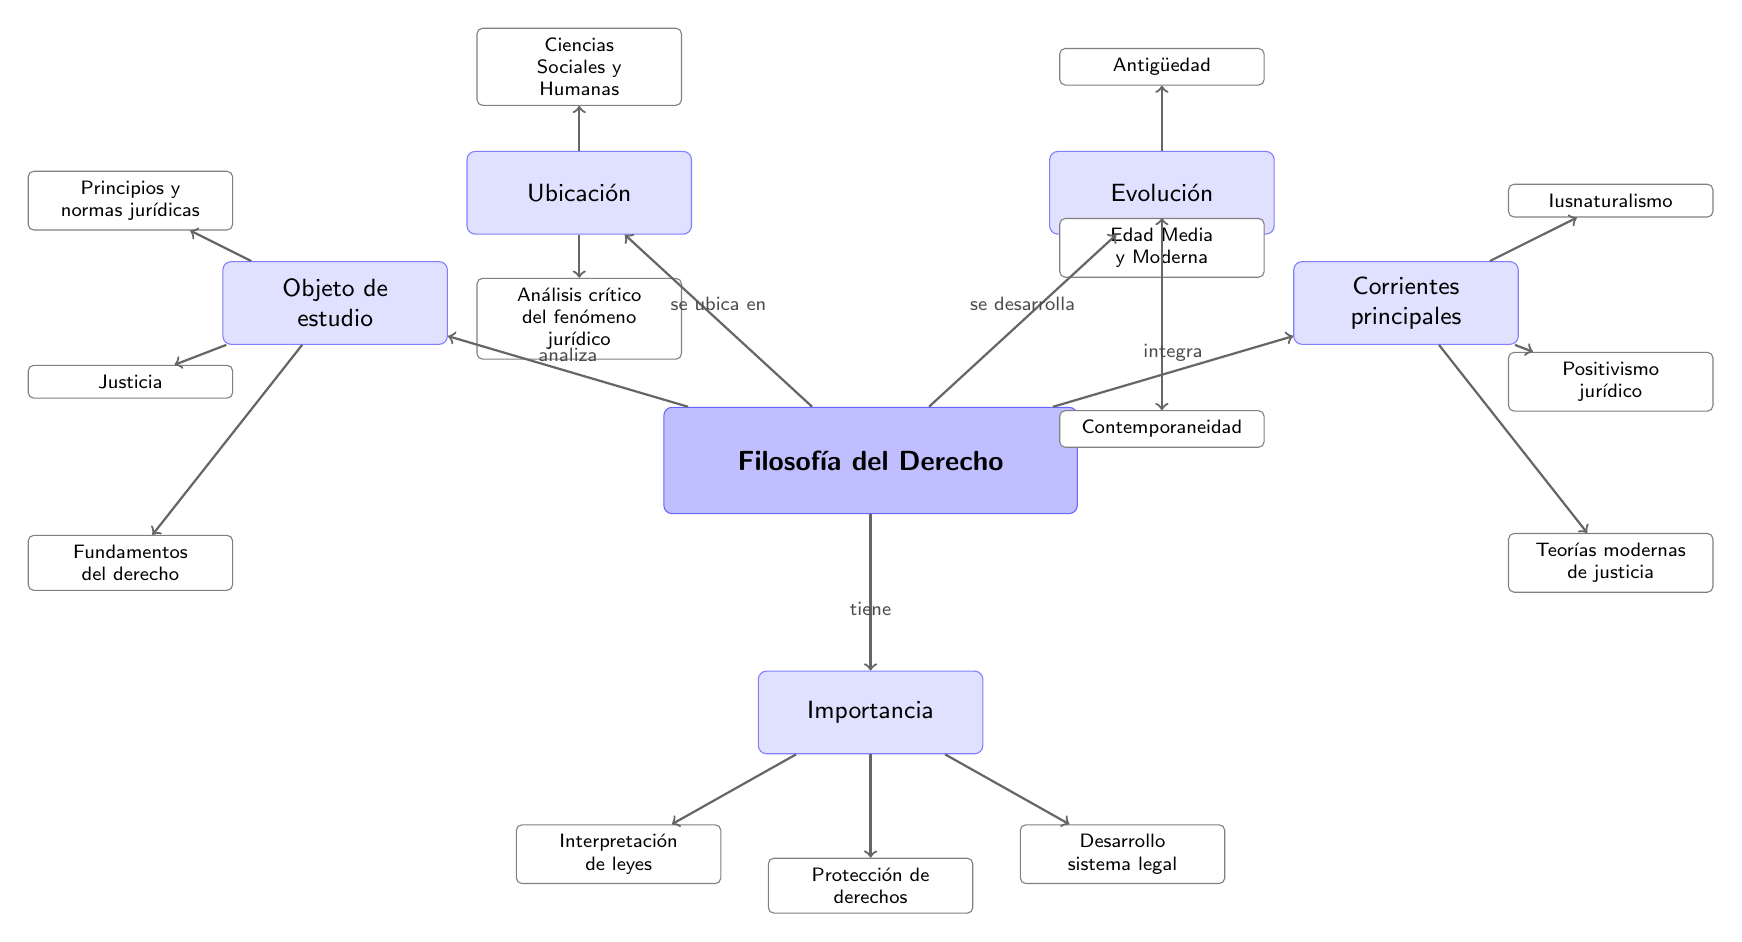
\begin{tikzpicture}[
	concept/.style={
		rectangle,
		rounded corners=3pt,
		draw=black!70,
		fill=gray!8,
		align=center,
		text width=3.0cm,
		minimum height=1.05cm,
		inner sep=5pt,
		font=\sffamily\small
	},
	root/.style={
		concept,
		fill=blue!25,
		draw=blue!60,
		text width=4.9cm,
		minimum height=1.35cm,
		font=\bfseries\sffamily\normalsize
	},
	branch/.style={
		concept,
		fill=blue!12,
		draw=blue!50,
		text width=2.5cm
	},
	subbranch/.style={
		rectangle,
		rounded corners=2pt,
		draw=black!50,
		fill=white,
		align=center,
		text width=2.35cm,
		inner sep=3.5pt,
		font=\sffamily\scriptsize
	},
	edge/.style={->,thick,black!60},
	label/.style={font=\sffamily\scriptsize,black!70}
]

% Nodo central
\node[root] (root) at (0,0) {\textbf{Filosofía del Derecho}};

% Rama 1: Objeto de estudio
\node[branch] (obj) at (-6.8,2.0) {Objeto de\\estudio};
\node[subbranch] (obj1) at (-9.4,3.3) {Principios y\\normas jurídicas};
\node[subbranch] (obj2) at (-9.4,1.0) {Justicia};
\node[subbranch] (obj3) at (-9.4,-1.3) {Fundamentos\\del derecho};

% Rama 2: Ubicación
\node[branch] (ubic) at (-3.7,3.4) {Ubicación};
\node[subbranch] (ubic1) at (-3.7,5.0) {Ciencias\\Sociales y\\Humanas};
\node[subbranch] (ubic2) at (-3.7,1.8) {Análisis crítico\\del fenómeno\\jurídico};

% Rama 3: Evolución
\node[branch] (evol) at (3.7,3.4) {Evolución};
\node[subbranch] (evol1) at (3.7,5.0) {Antigüedad};
\node[subbranch] (evol2) at (3.7,2.7) {Edad Media\\y Moderna};
\node[subbranch] (evol3) at (3.7,0.4) {Contemporaneidad};

% Rama 4: Corrientes
\node[branch] (corr) at (6.8,2.0) {Corrientes\\principales};
\node[subbranch] (corr1) at (9.4,3.3) {Iusnaturalismo};
\node[subbranch] (corr2) at (9.4,1.0) {Positivismo\\jurídico};
\node[subbranch] (corr3) at (9.4,-1.3) {Teorías modernas\\de justicia};

% Rama 5: Importancia
\node[branch] (imp) at (0,-3.2) {Importancia};
\node[subbranch] (imp1) at (-3.2,-5.0) {Interpretación\\de leyes};
\node[subbranch] (imp2) at (0,-5.4) {Protección de\\derechos};
\node[subbranch] (imp3) at (3.2,-5.0) {Desarrollo\\sistema legal};

% Conexiones rama 1
\draw[edge] (root) -- node[label,above]{analiza} (obj);
\draw[edge] (obj) -- (obj1);
\draw[edge] (obj) -- (obj2);
\draw[edge] (obj) -- (obj3);

% Conexiones rama 2
\draw[edge] (root) -- node[label,above]{se ubica en} (ubic);
\draw[edge] (ubic) -- (ubic1);
\draw[edge] (ubic) -- (ubic2);

% Conexiones rama 3
\draw[edge] (root) -- node[label,above]{se desarrolla} (evol);
\draw[edge] (evol) -- (evol1);
\draw[edge] (evol) -- (evol2);
\draw[edge] (evol) -- (evol3);

% Conexiones rama 4
\draw[edge] (root) -- node[label,above]{integra} (corr);
\draw[edge] (corr) -- (corr1);
\draw[edge] (corr) -- (corr2);
\draw[edge] (corr) -- (corr3);

% Conexiones rama 5
\draw[edge] (root) -- node[label,below]{tiene} (imp);
\draw[edge] (imp) -- (imp1);
\draw[edge] (imp) -- (imp2);
\draw[edge] (imp) -- (imp3);

\end{tikzpicture}
}%
\caption{Mapa Conceptual de la Filosofía del Derecho - Semana 2}
\label{fig:mapa-conceptual-filosofia}
\end{figure}

\vspace{-0.5cm}
\end{landscape}

% ======================= INICIO DEL DOCUMENTO =======================

\section{Introducción}

\begin{flushleft}
La Filosofía del Derecho es una disciplina fundamental que se encarga de analizar los principios, fundamentos y estructuras conceptuales del derecho. A través de esta actividad, se busca comprender los elementos esenciales que configuran el pensamiento jurídico, desde sus orígenes hasta las corrientes contemporáneas.

El presente trabajo tiene como objetivo identificar y mapear conceptualmente los aspectos clave de la Filosofía del Derecho, tales como su objeto de estudio, ubicación dentro del sistema de ciencias, evolución histórica, principales corrientes de pensamiento e importancia en la práctica jurídica actual.

Para lograr esto, se realizará una revisión exhaustiva de la bibliografía propuesta, se identificarán los conceptos fundamentales y se elaborará un mapa conceptual que sintetice estas ideas de manera clara y visual. Esta actividad permitirá desarrollar una comprensión crítica sobre la influencia de la filosofía jurídica en la estructura y evolución del sistema legal.
\end{flushleft}

\section{Conceptos Fundamentales de la Filosofía del Derecho}

A continuación, se presentan los conceptos clave identificados en la lectura del material, organizados en las siguientes categorías:

\begin{itemize}
	\item \textbf{Objeto de estudio:} Los principios, normas y sistemas jurídicos, así como los fundamentos de la justicia y el derecho natural \cite{finnis_estudios_2017,lovon_manual_2020}
	\item \textbf{Ubicación:} Disciplina dentro de las ciencias sociales y humanas que analiza críticamente el fenómeno jurídico \cite{ruiz_rodriguez_filosofia_derecho_2009}
	\item \textbf{Evolución:} Desarrollo histórico desde la antigüedad hasta la contemporaneidad, con énfasis en las teorías iusnaturalistas y positivistas
	\item \textbf{Corrientes:} Principales escuelas de pensamiento jurídico, incluyendo iusnaturalismo, positivismo jurídico y teorías modernas de justicia \cite{finnis_estudios_2017,ruiz_rodriguez_filosofia_derecho_2009,lovon_manual_2020}
	\item \textbf{Importancia:} Aplicación práctica en la interpretación y evolución del derecho, así como en los sistemas de protección de derechos fundamentales \cite{noauthor_constitucion_nodate,generales_ley_2021}
\end{itemize}

\subsection{Fundamentos Teóricos Identificados}

Según la bibliografía analizada:

\paragraph{Derecho Natural y Justicia}
El enfoque de Finnis en los estudios de teoría del derecho natural es fundamental para comprender cómo los principios universales de justicia y equidad configuran los sistemas legales \cite{finnis_estudios_2017}. Esta perspectiva contrasta con el positivismo jurídico pero ambas corrientes son esenciales para la comprensión integral de la filosofía del derecho.

\paragraph{Fundamentos Prácticos}
Lovón enfatiza la importancia de los fundamentos prácticos del derecho y la justicia, vinculando la teoría filosófica con la aplicación real en sistemas legales \cite{lovon_manual_2020}. Esto se refleja en los textos legales mexicanos como la Constitución Política, la Ley de Amparo, la Ley General de Víctimas y la Ley de Acceso de las Mujeres a una Vida Libre de Violencia \cite{noauthor_constitucion_nodate,generales_ley_2021,de_victimas_ley_2013,franzoni_acevedo_ley_2017}.

\paragraph{Principios Fundamentales}
Los textos legales mexicanos revelan principios clave como:
\begin{itemize}
	\item Legalidad y constitucionalidad
	\item Justicia y equidad
	\item Protección de derechos fundamentales
	\item Acceso a la justicia
	\item Reparación de víctimas
\end{itemize}

\section{Estructura Conceptual: Análisis de Elementos Fundamentales}

\subsection{Objeto de Estudio}

Según la bibliografía analizada, el objeto de estudio de la Filosofía del Derecho incluye:

\begin{enumerate}
	\item \textbf{Principios Jurídicos}: Son los principios que rigen la actividad jurídica y que sirven como base para la interpretación y aplicación de las normas legales. Estos principios pueden incluir la legalidad, la justicia, la equidad, entre otros \cite{finnis_estudios_2017,lovon_manual_2020}.
	\item \textbf{Normas y Sistemas Legales}: Son las reglas y principios que rigen el comportamiento humano en el ámbito jurídico, establecidas por autoridades competentes y que tienen efecto vinculante \cite{rojas_gonzalez_filosofia_derecho_2018,gandara_ley_2015}.
	\item \textbf{Justicia}: Es el principio moral y legal que busca la equidad en la distribución de bienes y servicios dentro de una sociedad \cite{finnis_estudios_2017,lovon_manual_2020}.
	\item \textbf{Fundamentos del Derecho}: Son los principios básicos que sustentan la existencia y funcionamiento del sistema jurídico \cite{ruiz_rodriguez_filosofia_derecho_2009,gandara_ley_2015}.
\end{enumerate}

\subsection{Corrientes Principales}

Las principales corrientes filosóficas en el estudio del derecho son:

\begin{enumerate}
	\item \textbf{Derecho Natural}: Esta corriente sostiene que existen principios universales de justicia y derecho que son inherentes a la naturaleza humana y que deben ser respetados por los sistemas legales \cite{finnis_estudios_2017}.
	\item \textbf{Positivismo Jurídico}: Esta corriente sostiene que el derecho es un conjunto de normas creadas por la autoridad competente y que no necesariamente están vinculadas a principios morales \cite{ruiz_rodriguez_filosofia_derecho_2009}.
	\item \textbf{Teorías Modernas de Justicia}: Estas teorías buscan integrar elementos de ambas corrientes anteriores, enfatizando la importancia de la equidad y la protección de derechos fundamentales en el sistema jurídico contemporáneo \cite{lovon_manual_2020,gandara_ley_2015}.
\end{enumerate}

\subsection{Elementos Fundamentales}

Los elementos fundamentales identificados son:

\begin{enumerate}
	\item \textbf{Derechos Fundamentales}: Son los derechos básicos e inalienables que todo ser humano posee, y que deben ser protegidos por el sistema jurídico \cite{noauthor_constitucion_nodate,generales_ley_2021}.
	\item \textbf{Principios Éticos}: Son los valores morales que guían la conducta humana y que influyen en la creación y aplicación de las normas legales \cite{finnis_estudios_2017,lovon_manual_2020}.
	\item \textbf{Ordenamiento Legal}: Es el conjunto de normas jurídicas que regulan la convivencia social y que son aplicadas por las autoridades competentes \cite{rojas_gonzalez_filosofia_derecho_2018}.
	\item \textbf{Instituciones Jurídicas}: Son las organizaciones y estructuras que facilitan la administración de justicia y la aplicación del derecho \cite{gandara_ley_2015}.
\end{enumerate}

\subsection{Aplicaciones Prácticas}

Las aplicaciones prácticas de la Filosofía del Derecho incluyen:

\begin{enumerate}
	\item \textbf{Sistema Constitucional (México)}: Es el marco legal que establece los derechos y obligaciones de los ciudadanos y las autoridades, y que sirve como base para la interpretación y aplicación de las normas legales \cite{noauthor_constitucion_nodate}.
	\item \textbf{Mecanismos de Protección}: Son los instrumentos legales que permiten a los ciudadanos defender sus derechos fundamentales ante posibles violaciones por parte de autoridades o particulares \cite{generales_ley_2021,de_victimas_ley_2013,franzoni_acevedo_ley_2017}.
	\item \textbf{Solución de Controversias}: Son los métodos alternativos para resolver conflictos legales sin necesidad de acudir a un proceso judicial formal, como la mediación o el arbitraje \cite{gandara_ley_2015}.
\end{enumerate}

\section{Conclusión}

Con base en el análisis de la bibliografía especializada en Filosofía del Derecho, se ha logrado identificar y sintetizar los conceptos fundamentales que configuran esta disciplina como un campo esencial de estudio en las ciencias sociales y humanas.

\paragraph{Hallazgos Principales:}

\begin{enumerate}
	\item \textbf{La Filosofía del Derecho como disciplina integral}: No se limita únicamente al análisis teórico, sino que integra tanto perspectivas iusnaturalistas como positivistas, generando un diálogo crítico que enriquece la comprensión del fenómeno jurídico \cite{finnis_estudios_2017,ruiz_rodriguez_filosofia_derecho_2009,lovon_manual_2020}.
	
	\item \textbf{Principios universales y contextos particulares}: Aunque existen principios universales de justicia y derecho natural, su manifestación concreta varía según el contexto histórico, social y cultural. El caso mexicano evidencia esto a través de sus marcos legales \cite{noauthor_constitucion_nodate,generales_ley_2021,de_victimas_ley_2013}.
	
	\item \textbf{Aplicabilidad práctica del conocimiento filosófico-jurídico}: La filosofía del derecho no es una disciplina puramente especulativa, sino que tiene profundas implicaciones en la estructura y funcionamiento de los sistemas legales contemporáneos, especialmente en la protección de derechos fundamentales y en mecanismos de justicia alternativa \cite{gandara_ley_2015}.
	
	\item \textbf{Importancia de la justicia como eje central}: La justicia emerge como el concepto vertebral de la filosofía del derecho, articulando los principios, normas y prácticas en un sistema coherente orientado hacia la equidad y protección de derechos.
\end{enumerate}

\paragraph{Relevancia Contemporánea:}

La actual legislación mexicana referente a protección de víctimas, derechos de las mujeres y mecanismos de solución alternativa de controversias refleja la evolución y aplicación práctica de los principios filosóficos del derecho en respuesta a demandas sociales contemporáneas \cite{de_victimas_ley_2013,franzoni_acevedo_ley_2017,gandara_ley_2015}.

En conclusión, la Filosofía del Derecho representa un campo de conocimiento interdisciplinario, crítico y reflexivo que proporciona las herramientas conceptuales necesarias para comprender, analizar y transformar los sistemas de justicia hacia una mayor equidad y protección de derechos fundamentales en la sociedad.

\clearpage

% \bibliography{UnADM}

\begin{thebibliography}{99}

% Referencias principales - Formato APA 7

\bibitem[Finnis et al.(2017)]{finnis_estudios_2017}
Finnis, J., Saldaña Serrano, J., \& Massini Correas, C. I. (2017). \textit{Estudios de teoría del derecho natural}. Universidad Nacional Autónoma de México, Instituto de Investigaciones Jurídicas.

\bibitem[Lovón(2020)]{lovon_manual_2020}
Lovón, J. F. (2020). \textit{Manual práctico de filosofía del derecho: fundamentos del derecho y justicia}. J. M. Bosch Editor.

\bibitem[Rojas González(2018)]{rojas_gonzalez_filosofia_derecho_2018}
Rojas González, G. (2018). \textit{Filosofía del derecho}. Editorial Universidad Católica de Colombia.

\bibitem[Ruiz Rodríguez(2009)]{ruiz_rodriguez_filosofia_derecho_2009}
Ruiz Rodríguez, V. (2009). \textit{Filosofía del derecho}. Instituto Electoral del Estado de México.

\bibitem[Constitución Política de los Estados Unidos Mexicanos(1917)]{noauthor_constitucion_nodate}
Constitución Política de los Estados Unidos Mexicanos. (1917). Diario Oficial de la Federación.

\bibitem[Ley de Amparo(2021)]{generales_ley_2021}
Ley de Amparo, Reglamentaria de los artículos 103 y 107 de la Constitución Política de los Estados Unidos Mexicanos. (2021). Diario Oficial de la Federación.

\bibitem[Ley General de Víctimas(2013)]{de_victimas_ley_2013}
Ley General de Víctimas. (2013). Diario Oficial de la Federación.

\bibitem[Franzoni Acevedo(2017)]{franzoni_acevedo_ley_2017}
Franzoni Acevedo, G. (2017). Ley General de Acceso de las Mujeres a una Vida Libre de Violencia: Importancia, evolución y dificultades. \textit{Entretextos: Revista Literaria y Cultural, 11}(24), 1--15.

\bibitem[Gándara Vásquez(2015)]{gandara_ley_2015}
Gándara Vásquez, C. A. (2015). \textit{Ley nacional de mecanismos alternativos de solución de controversias en materia penal}. Universidad de Xalapa.

\end{thebibliography}

% FIN DEL DOCUMENTO
\end{document}